\documentclass[a4paper]{article}
\usepackage{fullpage}
\usepackage[utf8]{inputenc}
\usepackage[english]{babel}

\usepackage[numbers]{natbib}
\usepackage[titletoc,toc,title]{appendix}
\usepackage{amsmath}
\usepackage{numprint}
\usepackage{graphicx}
\usepackage{titlesec}
\usepackage{tikz} \usetikzlibrary{trees, positioning, arrows.meta}
\usepackage{float}
\usepackage{listings}
\usepackage{xspace}
\usepackage{url}
\usepackage{hyperref}
\lstset{% parameters for all code listings
  language=Python,
  frame=single,
  columns=fullflexible,
  basicstyle=\small
}
\usepackage[autostyle]{csquotes} % fixes quote directions
\MakeOuterQuote{"}

% figure numbers reset each section
\usepackage{chngcntr}
\counterwithin{figure}{section}
\counterwithin{equation}{section}

% Custom macro for including images, \mfigure{img-name}{caption}
\newcommand{\mfigure}[2]{
\begin{figure}[H]
    \centering
    \includegraphics[width=\textwidth,height=0.30\textheight,keepaspectratio]{figures/#1.jpg}
    \caption{#2}
    \label{fig:#1}
\end{figure}
}

\begin{document}

\begin{titlepage}
\begin{center}
\includegraphics[height = 5cm, width = 5cm]{Uppsala.png} \\
\makeatletter
\vspace*{0.8cm}
\vspace{1 cm}
\textsc{\Large Uppsala University\\ }
\textsc{\large Analysis of Crimes in Chicago\\}
\textsc{\large Large DataSet for Scientific Applications}
\textsc{\Large}\\[0.3cm]
\textnormal{\large Project Report by Group 12}\\
\textnormal{Ankur Shukla}\\
\textnormal{Arianna Delsante}\\
\textnormal{Lukas Enander}\\
\textnormal{Santhosh Kumar Nagarajan}\\
\textnormal{\\\today}
% Bottom of the page
\end{center}
\end{titlepage}


\section{Background}
% TODO :Description of the scientific area/problem that gave rise to the dataset. Place the dataset in context, providing sufficient references for the reader to understand the importance and significance of the data. What kind of analyses have been done in the literature?

The chosen dataset contains reported crimes in the City of Chicago from the year 2001 to present, except for the last seven days. The data is generated by the Chicago Police Department’s CLEAR (Citizen Law Enforcement Analysis and Reporting) system, which is a system for government agencies in the Chicago area to share information about crime and criminal records \cite{CLEARpolice}. CLEAR is not available to the public, but parts of it is published in the Chicago Open Data Portal, provided by the city of Chicago, which was the source for the dataset used in this project. 

The specific dataset used is called “Crimes - 2001 to present” and is presented under the “Public Safety” category of the Chicago Open Data Portal and contains approximately 6,6 million reported crimes during the time period. The data is showing details such as crime type, date, location, arrest and more. An exact address is not provided in this public dataset for privacy reasons, but the street block address is provided for approximate geographical location \cite{cityOfChicago}. 

The Chicago Open Data Portal has done some analyses on the data already which is provided as graphs in the portal for easy overview. Theses include the aggregated number of crimes per month for the whole time period to show the trend in reported crimes over time. Other than that, graphs counting crimes by primary type, arrest percentage, domestic or non domestic and maps showing crime rate in different police districts and zip codes are presented. 
\section{Data Format}

%TODO: Describe the data format(s) used in the dataset. Put them in context: why were the specific formats chosen, and would there be alternatives? What are the pros and cons of the formats used?
The Chicago dataset provides a farraginous data formats as listed below:
\begin{itemize}
    \item \textbf{CSV (Comma Separated Values)}: CSV format stores tabular data in 2 dimensions consisting of row(s) and column(s). Each row in the csv file is considered as a record. Data fields are separated by commas, the rows are separated by a new line\cite{csv}.
    \item \textbf{JSON (JavaScript Object Notation)}: JSON is a standard text-based format for representing structured data based. It is widely used for transmitting data in web applications\cite{json}.
    \item \textbf{RDF (Resource Description Framework)}: RDF framework is written in XML for describing the resources on the web; it allows effective data integration from multiple data objects\cite{rdf}.
    \item \textbf{RSS (Rich Site Summary)}: RSS is a Syndication Standard based on a type of XML file that resides on an Internet server. RSS is formally known as Really Simple Syndication\cite{rss}.
    \item \textbf{XML (Extensible Markup Language)}: XML file format is used to create common information formats and share both the format and the data on the web \cite{xml}.
\end{itemize}

We used Spark for analyzing the city of Chicago dataset to find ‘the frequency of crime over crime categories’. In Chicago dataset, the published crime records are in structured format. It is much more convenient to relate columns in structured format. We have chosen “CSV” format to analysis the inter-related fields.\newline
The CSV format offer us the following advantages\cite{csv_advantage}:
\begin{itemize}
    \item CSV file follows simple schema, it can be opened or edited by text editors and manipulated programmatically at ease.
    \item Importing CSV file is much faster and consumes less memory.
    \item CSV is compact. For example in XML you need to start a tag and end the tag for each column in each row. However in CSV format you write the column headers only once.
    \item CSV is feasible for sending huge data amounts with less bandwidth.
\end{itemize}

It requires to build a parsing and containing structure for CSV, while XML DOM provides an inherent structure. XML provides data hierarchy where it is convenient to query a data field; CSV does not support data hierarchies. JSON is more compact and easier to work with data at scale\cite{json_advantage}.







\section{Computational Experiment}

%TODO: The main section of the report. Describe and motivate the choice of tools and the distributed system that you designed. Describe how you have designed your scalability experiments,and present the results.

This section provides the motivation for our choice of tools and briefly describes the distributed system that we designed. 

\subsection{Tools \& Implementations}
We are using Spark as it provides a new model of computation that allows to perform parallel operations on a specific set of data. In our project we apply multiple functions repeatedly to the same data set to extract various statistical information. Spark offers the possibility to improve performance significantly without reloading the data form disk each time \cite{Sparkzaharia}.The feature which supports much faster processing is in-memory computation.

Our dataset is read by collection of objects called RDD, these objects allow parallel operations with an option to cache an RDD in memory, so that it could be reused for other MapReduce operations. 

We are constructing RDD from a \textit{.csv} file using shared file system. The System we have is fault tolerant, in fact if a partition of an RDD is lost it is possible to rebuild just that partition given the information on how it was derived from other RDDs. This is called \textit{lineage}\cite{Sparkzaharia}.

In our system a \textit{driver program} connects to a cluster of \textit{workers}. These are processes that can store RDD partitions in RAM across operations\cite{RDD}.\newline
Our final code used pyspark RDD and dataframe for analyzing the dataset. We implemented a cluster with single worker node and tested it; so that we could abstract the data we wanted. When the implemented configuration was working correctly, we get to implement a cluster with a master node and 3 worker nodes.When we ran our code on 35 Gb dataset, it divides the data into 288 partitions and observed that the computation on 3 worker node consumed lesser time over the single worker node configuration; the observed values are represented in Figure \ref{fig:stages_three_fourth}. 

We created Virtual Machine at SNIC Science Cloud \cite{snic} and used the following settings:

\begin{itemize}
    \item \textbf{Source:} Volume Snapshot of 'snapshotgroup12'. We used the snapshot volume from SNIC to configure Spark environment.
    \item \textbf{Flavor:} $ssc.medium$ which had 2 VCPUs, 4Gb Ram, 40 Gb total disk and root disk
    \item \textbf{Networks:} SNIC 2018/10-13 Internal IPv4 Network.
    \item Our Cluster with 3 worker node has total of 6 cores(2 cores each) with the memory of 8.6 Gb(2.9 Gb each). You can see our Spark UI with 3 worker node in Figure \ref{fig:spark_master_three}. 
\end{itemize}

\begin{figure}[H]
    \centering
    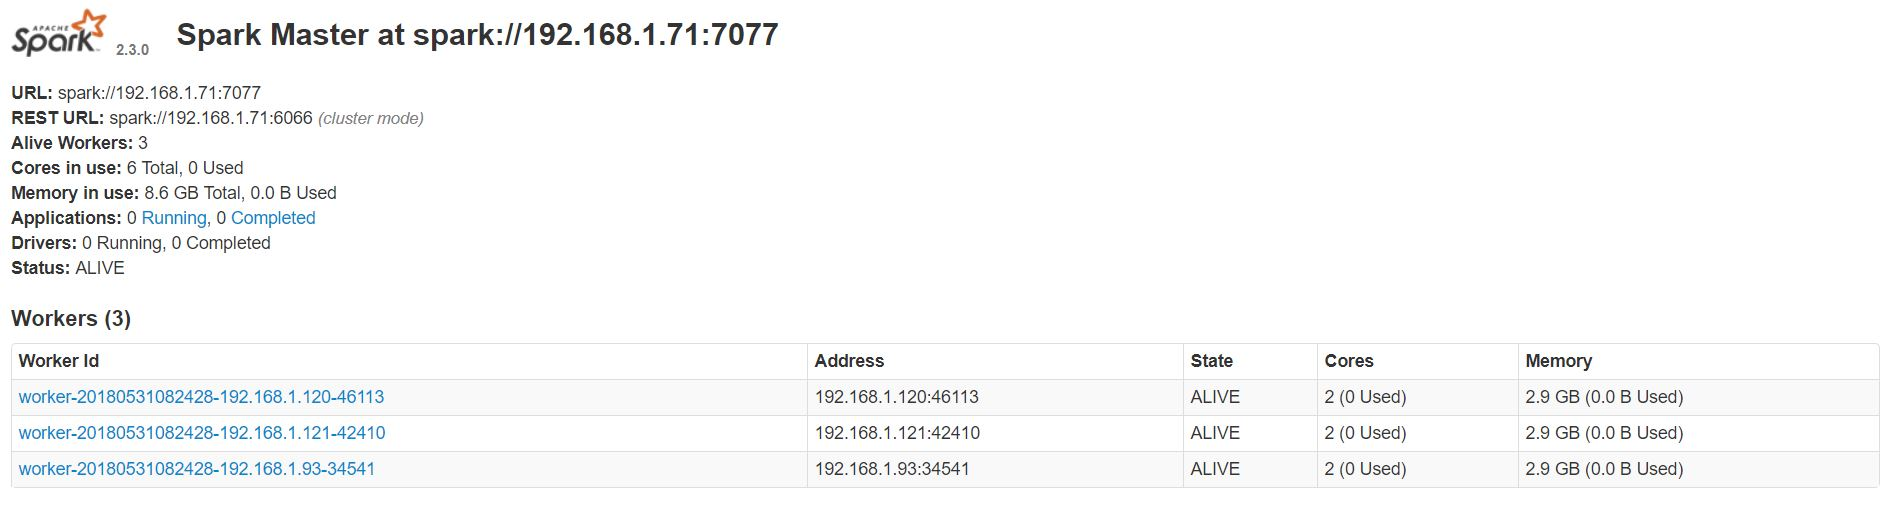
\includegraphics[width=.95\linewidth]{figures/spark_master_three.jpg}
    \caption{Screen-shot of our Spark UI Cluster with 3 worker nodes.}
    \label{fig:spark_master_three}
\end{figure}


\subsection{Results}
For this project, we used Chicago city Crimes data set\cite{cityOfChicago} and it contained many relevant information associated with each of the crime that has occurred in Chicago from year 2001 until now. We are plotting 4 different graphs associated with 4 different columns. A program in pyspark was created to plot these graph. You can look at the code \href{https://github.com/ankurshukla03/ldsaproject/blob/edit_report/code/Crimes.ipynb}{here.} \\
Below is 4 different plots presenting the results :\\

\mfigure{crime_type}{Plot representing the frequency of particular crime type that has occurred in Chicago from year 2001 until now. Our  generated plots seemed similar to the Figure \ref{fig:exampleGraph} which we took from Chicago portal \cite{cityOfChicago}.}

\mfigure{month}{Plot representing the frequency of crime across the months.}

\mfigure{year}{Plot representing the frequency of crime per year.}

\mfigure{location}{Plot representing the frequency of crime with location description. Our plot is correct when compared with the plot in the dashboard of Chicago portal \href{https://data.cityofchicago.org/Public-Safety/Crimes-2001-to-present-Dashboard/5cd6-ry5g}{here.}}


\subsection{Scalability experiment}
In order to test and confirm the scalability of the system, scalability studies were conducted. Since the original dataset was only of 1,45 GB, it was scaled up by replicating it in order to get larger datasets. Four different sizes of the dataset were produced including the original one. These were 1.45 Gb, 11.2 Gb, 23.2 Gb and 35 Gb and you can see the time taken with different number of nodes on these data size in Table \ref{table_time}.

To measure the horizontal scalability, the run time for a specific job on the dataset were recorded for 1 and 3 nodes cluster configuration. As seen in  \ref{fig:scalabilityGraph} below we can observe that
the run time increased linearly with data size for the different cluster configurations and the run time was reduced equally for increasing number of nodes. Furthermore, the slopes for the linear fits of the data points are shown. The slope for one node is 41.241 s/GB and for four nodes it is 13.114 s/GB. This means that the second configuration is 3,15 times faster.\\

\begin{table}[]
    \centering
    \begin{tabular}{|c|c|c|}
\hline
Number of Nodes  & Time Taken & Data Size \\ \hline
        1 & 1.1 min & 1.45 Gb \\ \hline
        3 & 32 seconds & 1.45 Gb \\
\hline
\end{tabular}
\quad
\begin{tabular}{|c|c|c|}
\hline
Number of Nodes  & Time Taken & Data Size \\ \hline
        1 & 4.1 min & 5.8 Gb \\ \hline
        3 & 1.4 min & 5.8 Gb \\
\hline
\end{tabular}
\begin{tabular}{|c|c|c|}
\hline
Number of Nodes  & Time Taken & Data Size \\ \hline
        1 & 16 min & 23.2 Gb \\ \hline
        3 & 5.1 min & 23.2 Gb \\
\hline
\end{tabular}
\quad
\begin{tabular}{|c|c|c|}
\hline
Number of Nodes  & Time Taken & Data Size \\ \hline
        1 & 24 min & 35 Gb \\ \hline
        3 & 7.6 min & 35 Gb \\
\hline
\end{tabular}
    \caption{Time taken by reduce functionality using different cluster configuration over different data size.}
    \label{table_time}
\end{table}


\mfigure{stages_one_fourth}{Screenshot of our Spark UI stages tab when ran with 1 node on 35 Gb data size.}

\mfigure{stages_three_second}{Screenshot of our Spark UI stages tab when ran with 3 node on 5.8 Gb data size.}

\mfigure{stages_three_fourth}{Screenshot of our Spark UI stages tab when ran with 3 worker node on 35 Gb data size.}


\begin{figure}[H]
    \centering
    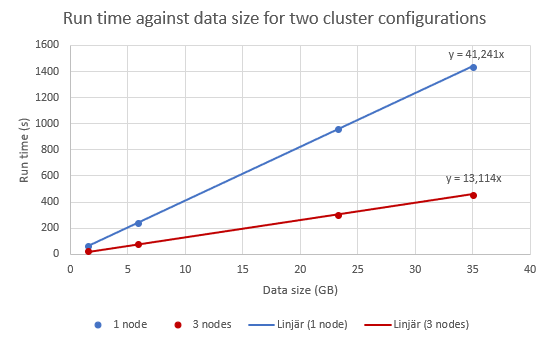
\includegraphics[width=.75\linewidth]{figures/runTime2.PNG}
    \caption{Run time for different data sizes plotted for two cluster configurations. Blue line denotes the cluster with one node and the red line denotes with three nodes.}
    \label{fig:scalabilityGraph}
\end{figure}


\section{Disussion and Conclusion}

%TODO: Here you can discuss the outcome of the experiments and the experiences gained. Was your chosen approach suitable? What worked well and what could be improved?

%outcome of the experiment?
We are satisfied with our results and they seem to be correct. When you compare them with the plots present in Chicago Crimes-2001 to present- dashboard \cite{chicago_location} and the graphs are right.
\bigbreak
%scalability of our code and experiences gained
%chosen approach suitable or not
As for the scalability experiments, both cluster configurations had a linear run time increase with increasing data size, indicating that the system scales well with regards to bigger data operations. In other words, doubling the data size also doubles the computational time, which is the wanted behaviour for this kind of system.

The run time decreased by a factor of 3,15 (31,8 \% of the original time) when increasing the number of nodes from one to three. This seems to indicate that the horizontal scalability of the system is very good, at least with relatively few nodes in the cluster. Why the run time decreased to less than a third... (dont know what to write here yet)
\bigbreak
In order to further examine the system and the scalability of it, more cluster configurations with different number of nodes could have been tested to determine if the result holds true even for these setups. It is possible that the behaviour of the system scales well on the small clusters tested here, but experiences diminishing returns as the number of nodes goes up further. It would be interesting to see at what number of nodes and data size that potentially could happen. 


%for citing any reference add it in the .bib file and cite it using \cite{} command and pass the name which you gave it in .bib file it will be generated in the latex report automatically
\bibliographystyle{plain}
\bibliography{references}
\end{document}
